O ambiente descrito no Capítulo \ref{cap:ambExperimental} foi utilizado para a realização das simulações e a ferramenta JMeter foi executada dentro do servidor Maritaca para evitar que o tempo de latência de Internet impactasse nos experimentos.

Em todas as simulações, o balanceamento de carga dos testes foi realizado automaticamente pelo JMeter e a criação dos dados a serem gravados foi feita utilizando uma função randômica do próprio simulador. A consistência de escrita dos dados era \textit{ONE}\footnote{Caracteriza a gravação dos dados em apenas um nó, sem replicação.} quando havia apenas um nó e \textit{TWO}\footnote{Caracteriza a gravação dos dados em um nó e replicação do mesmo em outro nó.} quando o \textit{cluster} possuia mais que um nó. 

Cada nó do \textit{cluster} de dados poderia receber até 100 conexões simultâneas e o tipo de cliente utilizado na conexão do simulador com a base de dados foi o \textit{ThriftConnection}, devido ao Cassandra utilizar este cliente como padrão.

O tempo de duração das requisições de cada teste foi de 60 segundos, sendo que entre cada um dos testes havia um intervalo de 30 segundos, no qual era feito o \textit{flush} dos dados gravados temporariamente pelo JMeter. Em todos os cenários testou-se o comportamento da base de dados Cassandra quando o acesso simultâneo de usuários variava de 1 a 4000 usuários.

\section{Cenário 1}

Neste cenário, as operações de inserção de dados no Cassandra foram realizadas com o Cassandra operando apenas com um nó.
Para isto, utilizou-se um \textit{host} contendo apenas o Cassandra instalado.

    \begin{figure}[H]
    \centering
    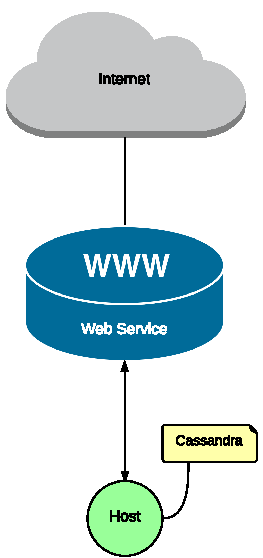
\includegraphics[scale=0.60]{imagens/BD-1Host.pdf}
    \caption{Cenário 1}
    \label{fig:bd1host}
    \end{figure} 

\section{Cenário 2}
Neste cenário, as operações de inserção de dados no Cassandra foram realizadas com o Cassandra operando apenas com um nó.
Para isto, utilizou-se um \textit{guest} contendo apenas o Cassandra instalado. O objetivo neste cenário era avaliar possíveis diferenças entre \textit{host} e \textit{guest}.

    \begin{figure}[H]
    \centering
    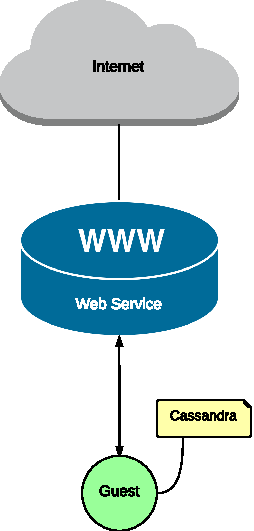
\includegraphics[scale=0.60]{imagens/BD-1Guest.pdf}
    \caption{Cenário 2}
    \label{fig:bd1guest}
    \end{figure} 

Com os cenários 1 e 2 buscou-se ver o comportamento e a carga suportada por esse ambiente para que pudéssemos compará-lo com o terceiro cenário.

\section{Cenário 3}
Neste cenário, as operações de inserção de dados no Cassandra foi realizada com o Cassandra operando com um \textit{cluster} contendo 2 nós.
Para isto, utilizou-se 2 \textit{host} contendo apenas o Cassandra instalado.
Essas mudanças visavam verificar a possível melhora no serviço oferecido com a inclusão de novas máquinas aos \textit{clusters}, utilizando-se assim da elasticidade presente nos ambientes de computação em nuvem.

    \begin{figure}[H]
    \centering
    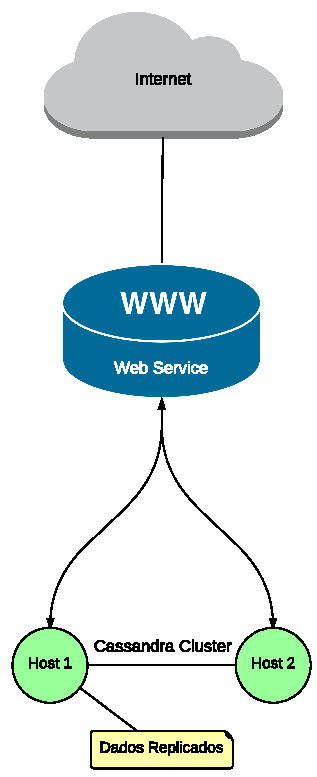
\includegraphics[scale=0.60]{imagens/BD-2Host.pdf}
    \caption{Cenário 3}
    \label{fig:bd2host}
    \end{figure} 
    
    
\section{Cenário 4}
Neste cenário, as operações de inserção de dados no Cassandra foi realizada com o Cassandra operando com um \textit{cluster} contendo 2 nós.
Para isto, utilizou-se 2 \textit{guest} contendo apenas o Cassandra instalado.
Com este cenário foi possível comparar a elasticidade entre ambientes configurados apenas com \textit{hosts} e em ambientes configurados apenas com \textit{guests}.

    \begin{figure}[H]
    \centering
    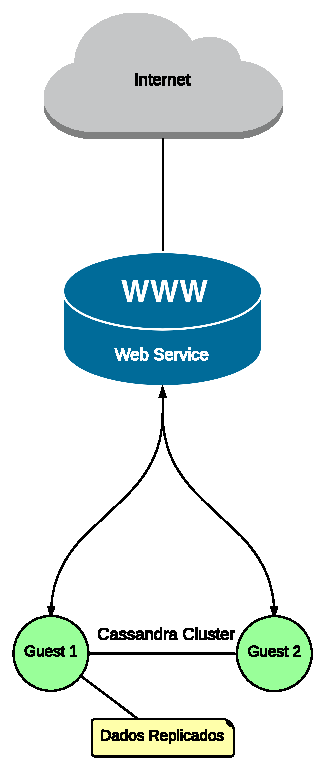
\includegraphics[scale=0.60]{imagens/BD-2Guest.pdf}
    \caption{Cenário 4}
    \label{fig:bd2guest}
    \end{figure} 


\section{Cenário 5}
Neste cenário, as operações de inserção de dados no Cassandra foram realizadas com o Cassandra operando com um \textit{cluster} contendo 2 nós.
Para isto, utilizou-se um \textit{host} e um \textit{guest} contendo apenas o Cassandra instalado, conforme a Figura \ref{fig:bd1host1guest}.

Essas mudanças visavam verificar a comunicação entre \textit{clusters} configurados mesclando \textit{hosts} e \textit{guests} e avaliar o serviço oferecido com a inclusão de novas máquinas aos clusters, utilizando-se assim da elasticidade presente nos ambientes de computação em nuvem.

    \begin{figure}[H]
    \centering
    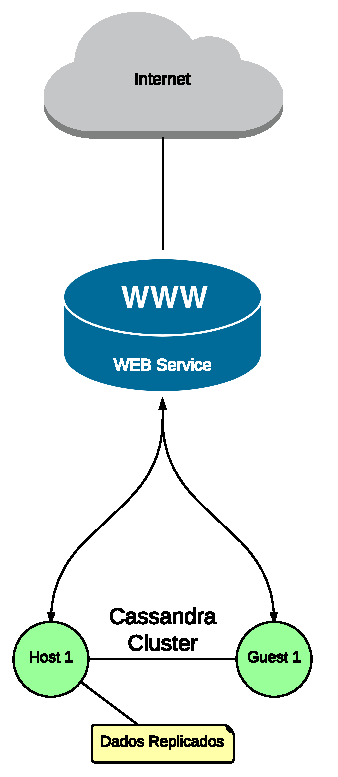
\includegraphics[scale=0.60]{imagens/BD-1Host1Guest.pdf}
    \caption{Cenário 5}
    \label{fig:bd1host1guest}
    \end{figure} 



\section{Cenário 6}
Para o último cenário, definiu-se uma configuração mais comum de observar em aplicações de grande porte, onde a elasticidade das \textit{guests} é utilizada em larga escala. Logo, as operações de inserção de dados no Cassandra foi realizada com o Cassandra operando com um \textit{cluster} contendo 4 nós.
Para isto, utilizou-se 4 \textit{guests} contendo apenas o Cassandra instalado.

    \begin{figure}[H]
    \centering
    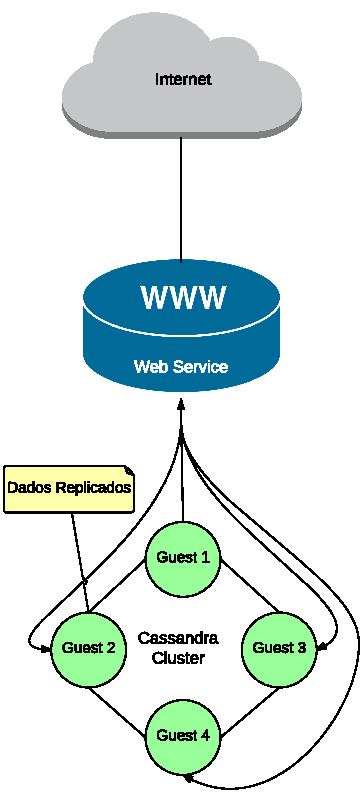
\includegraphics[scale=0.60]{imagens/BD-4Guest.pdf}
    \caption{Cenário 6}
    \label{fig:bd4guest}
    \end{figure}


\section{Resultados}

A Tabela \ref{tab:am} se refere a quantidade de pacotes gravados na base de dados, em 60 segundos.

\begin{table}[ht]
\centering
\caption{Quantidade de amostras gravadas}
\label{tab:am}
\begin{tabular}{|
>{\columncolor[HTML]{C0C0C0}}c |c|c|c|c|c|c|}
\hline
Usuários & \cellcolor[HTML]{C0C0C0}Cenário 1 & \cellcolor[HTML]{C0C0C0}Cenário 2 & \cellcolor[HTML]{C0C0C0}Cenário 3 & \cellcolor[HTML]{C0C0C0}Cenário 4 & \cellcolor[HTML]{C0C0C0}Cenário 5 & \cellcolor[HTML]{C0C0C0}Cenário 6 \\ \hline
1 & 6229 & 6178 & 6097 & 14689 & 7838 & 7126 \\ \hline
10 & 24053 & 34834 & 47324 & 43296 & 44783 & 45340 \\ \hline
50 & 30146 & 41400 & 46469 & 47060 & 44277 & 36392 \\ \hline
100 & 41831 & 42203 & 43928 & 43755 & 43316 & 35651 \\ \hline
250 & 39667 & 43661 & 40750 & 44406 & 40436 & 37234 \\ \hline
500 & 42179 & 39367 & 41925 & 43392 & 39206 & 37514 \\ \hline
750 & 40617 & 40840 & 37081 & 41931 & 41035 & 36169 \\ \hline
1000 & 40904 & 40669 & 37550 & 41995 & 40007 & 38508 \\ \hline
1250 & 40341 & 41916 & 40454 & 43294 & 39681 & 36632 \\ \hline
1500 & 39448 & 42382 & 38359 & 41300 & 38146 & 39555 \\ \hline
1750 & 41258 & 39857 & 37295 & 41564 & 40696 & 40452 \\ \hline
2000 & 42677 & 41467 & 37612 & 41544 & 38236 & 37361 \\ \hline
2250 & 43511 & 42758 & 39323 & 38937 & 39334 & 36440 \\ \hline
2500 & 39481 & 35500 & 32545 & 32982 & 30695 & 35017 \\ \hline
2750 & 36579 & 35517 & 31575 & 33886 & 29995 & 33270 \\ \hline
3000 & 34654 & 34590 & 32114 & 35230 & 32919 & 31941 \\ \hline
3250 & 36240 & 34824 & 31875 & 34220 & 31856 & 31560 \\ \hline
3500 & 33632 & 35368 & 33049 & 34827 & 31900 & 29891 \\ \hline
3750 & 28991 & 36347 & 34037 & 36161 & 33386 & 24095 \\ \hline
4000 & 26672 & 34773 & 34672 & 33493 & 33339 & 20970 \\ \hline
\end{tabular}
\end{table}

Após tabulados os dados, plotou-se o gráfico exibido na Figura \ref{fig:am} para possibilitar uma melhor avaliação dos resultados.




    \begin{figure}[!h]
    \centering
    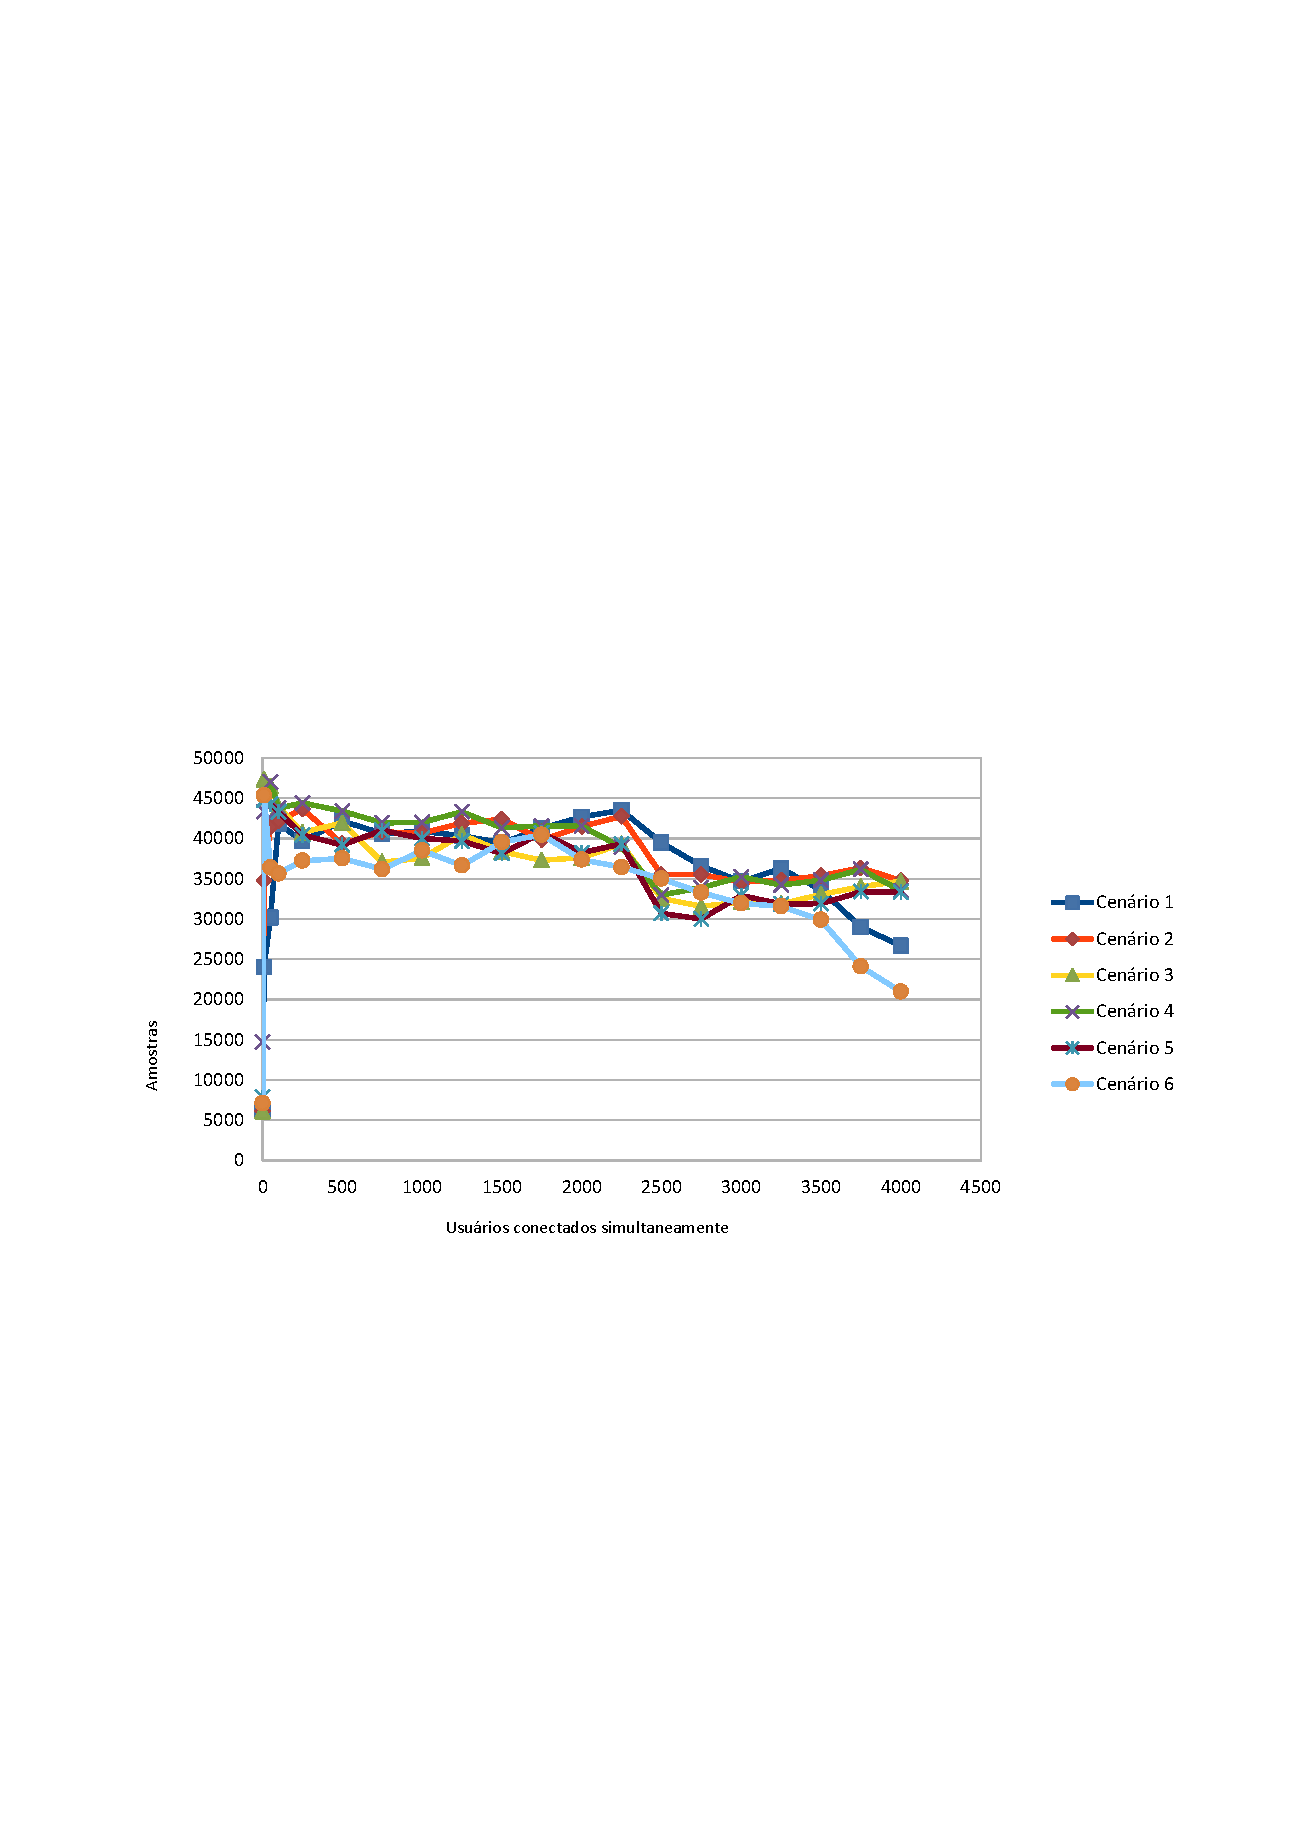
\includegraphics[scale=0.85]{imagens/amXmin.pdf}
    \caption{Quantidade de amostras gravadas por minuto}
    \label{fig:am}
    \end{figure}

Também analisou-se a quantidade de erros gerado com aumento do número de usuários, conectados simultaneamente à base de dados Cassandra, conforme a Tabela \ref{tab:erro}.


\begin{table}[ht]
\centering
\caption{Porcentagem de erro na gravação de pacotes}
\label{tab:erro}
\begin{tabular}{|
>{\columncolor[HTML]{C0C0C0}}c |c|c|c|c|c|c|}
\hline
Usuários & \cellcolor[HTML]{C0C0C0}Cenário 1 & \cellcolor[HTML]{C0C0C0}Cenário 2 & \cellcolor[HTML]{C0C0C0}Cenário 3 & \cellcolor[HTML]{C0C0C0}Cenário 4 & \cellcolor[HTML]{C0C0C0}Cenário 5 & \cellcolor[HTML]{C0C0C0}Cenário 6 \\ \hline
1 & 0 & 0 & 0 & 0 & 0 & 0 \\ \hline
10 & 0 & 0 & 0 & 0 & 0 & 0 \\ \hline
50 & 0 & 0 & 0 & 0 & 0 & 0 \\ \hline
100 & 0 & 0 & 0 & 0 & 0 & 0 \\ \hline
250 & 0 & 0 & 0 & 0 & 0 & 0 \\ \hline
500 & 0 & 0 & 0 & 0 & 0 & 0 \\ \hline
750 & 0 & 0 & 0 & 0 & 0 & 0 \\ \hline
1000 & 0 & 0 & 0 & 0 & 0 & 0 \\ \hline
1250 & 0 & 0 & 0 & 0 & 0 & 0 \\ \hline
1500 & 0 & 0 & 0 & 0 & 0 & 0 \\ \hline
1750 & 0 & 0 & 0 & 0 & 0 & 0 \\ \hline
2000 & 0 & 0 & 0 & 0 & 0 & 0 \\ \hline
2250 & 10 & 0 & 0 & 8 & 0 & 3 \\ \hline
2500 & 16 & 13 & 19 & 20 & 24 & 9 \\ \hline
2750 & 17 & 16 & 21 & 21 & 27 & 14 \\ \hline
3000 & 15 & 15 & 19 & 18 & 23 & 15 \\ \hline
3250 & 13 & 13 & 17 & 16 & 20 & 15 \\ \hline
3500 & 22 & 12 & 15 & 14 & 18 & 22 \\ \hline
3750 & 30 & 11 & 14 & 13 & 16 & 36 \\ \hline
4000 & 37 & 12 & 13 & 20 & 16 & 46 \\ \hline
\end{tabular}
\end{table}


Os erros de gravação foram plotados variando o cenário utilizado e a quantidade de usuários, conforme a Figura \ref{fig:erro}. 


    \begin{figure}[H]
    \centering
    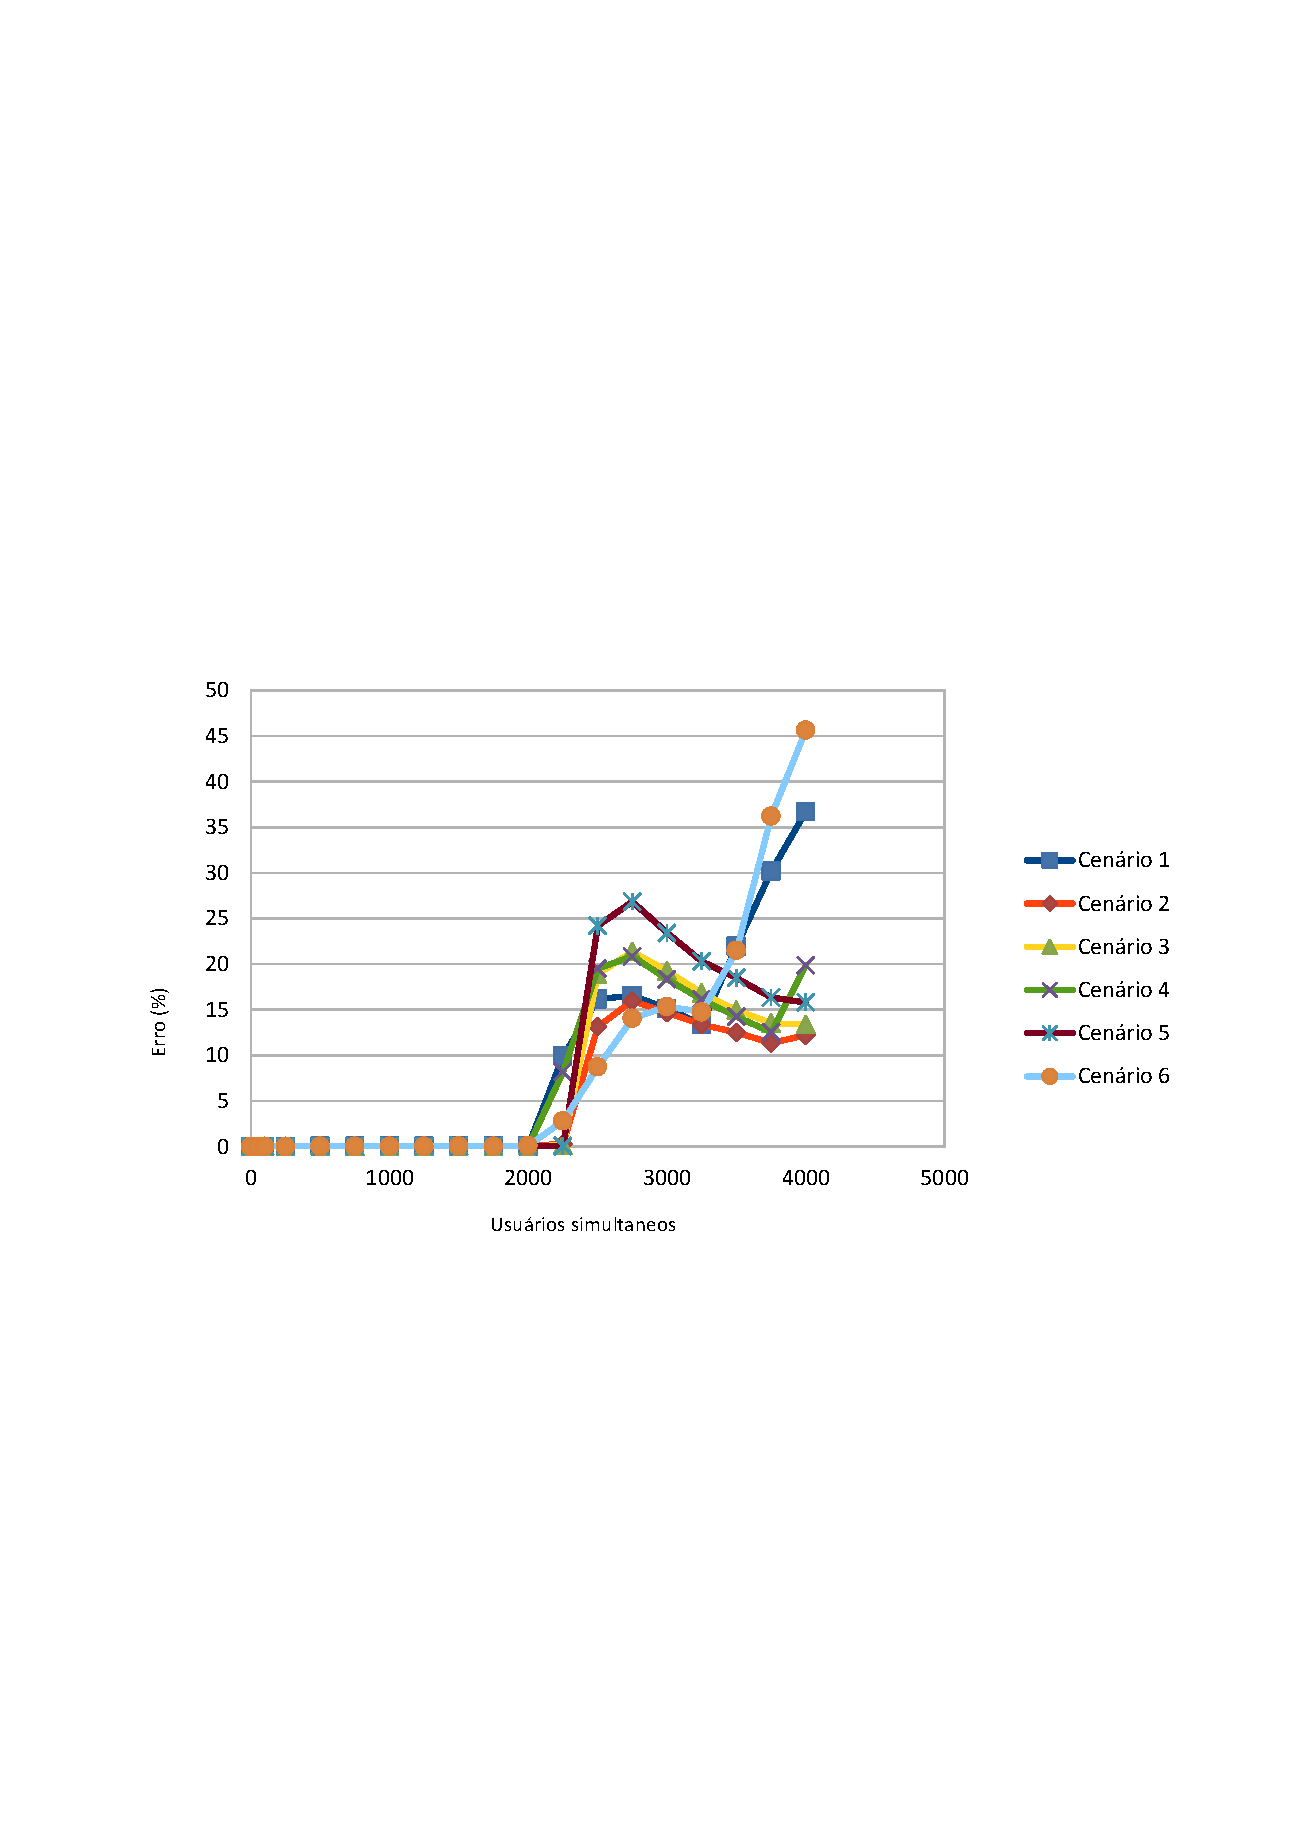
\includegraphics[scale=0.85]{imagens/erroXmin.pdf}
    \caption{Porcentagem de erro na gravação de pacotes}
    \label{fig:erro}
    \end{figure}
    
    
Com os dados obtidos nestas duas avaliações iniciais (Figura \ref{fig:am} e \ref{fig:erro}), não foi possível observar a escalabilidade da base de dados, porém, notou-se que a partir de 2000 usuários, todos os cenários tiveram um aumento considerável do número de erros e consequentemente uma diminuição do número de requisições atendidas com sucesso. 

Este comportamento também foi notado em todos os gráficos de média e desvio padrão, nos quais houve um aumento expressivo do desvio padrão a partir desta quantidade de usuários, conforme as Figuras \ref{fig:dvp1}, \ref{fig:dvp2}, \ref{fig:dvp3}, \ref{fig:dvp4}, \ref{fig:dvp5} e \ref{fig:dvp6}. 

    \begin{figure}[H]
    \centering
    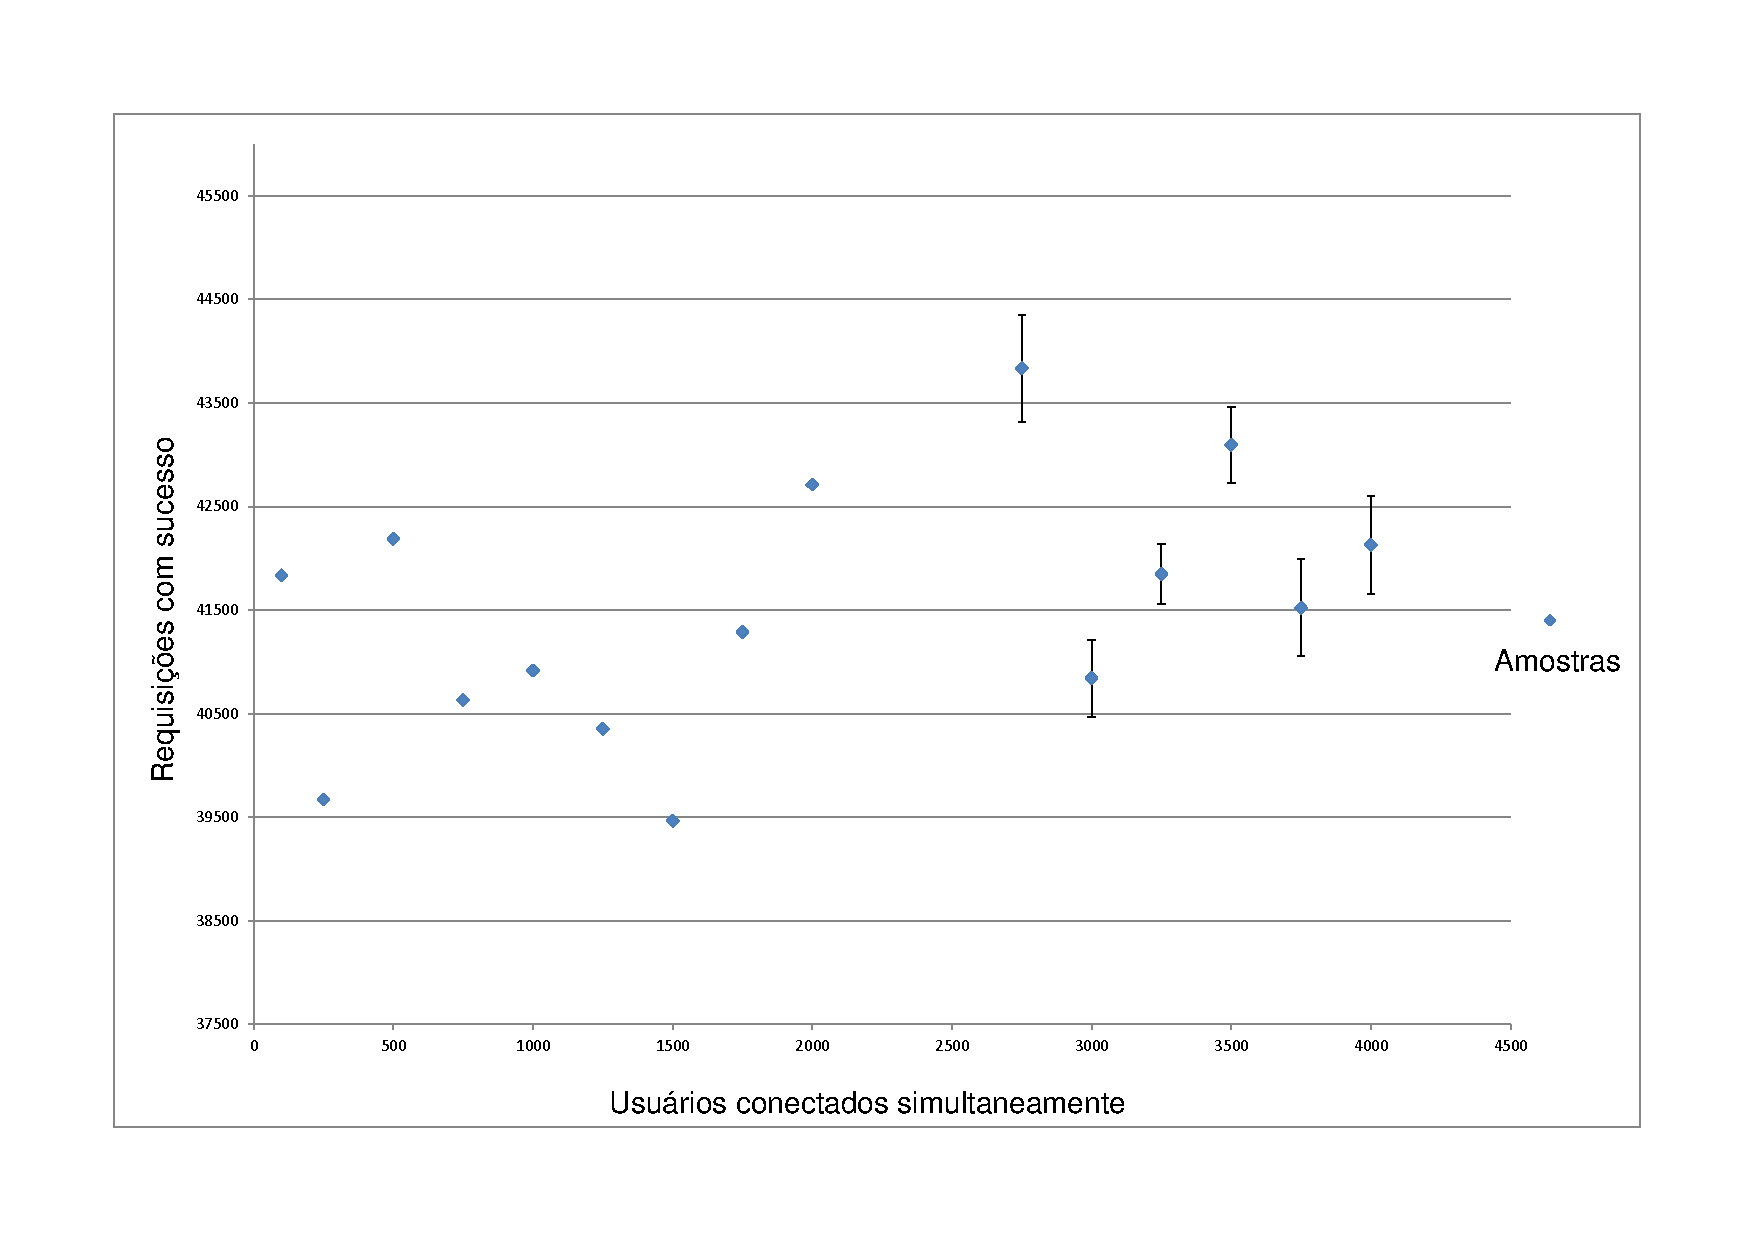
\includegraphics[scale=0.50]{imagens/dvp1.pdf}
    \caption{Média e desvio padrão do Cenário 1}
    \label{fig:dvp1}
    \end{figure}
    
        \begin{figure}[H]
    \centering
    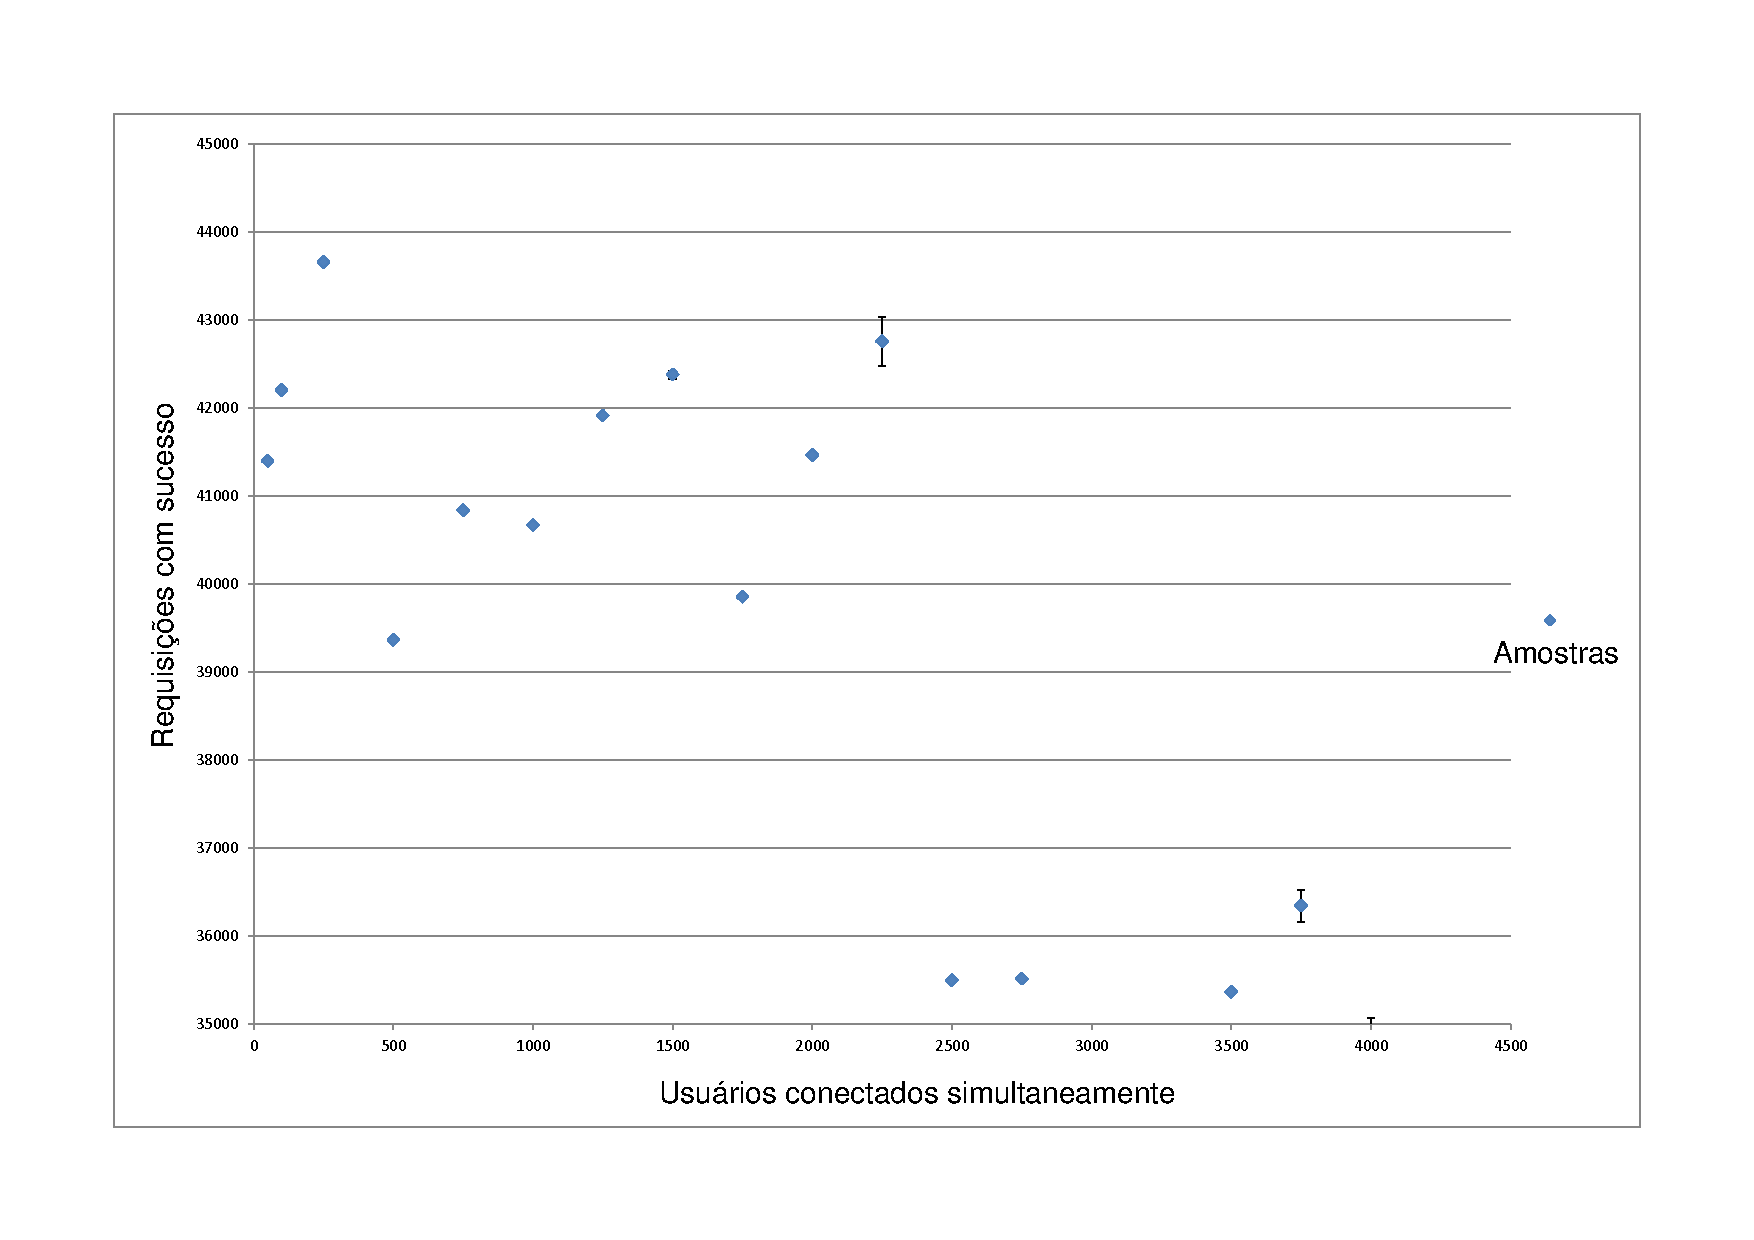
\includegraphics[scale=0.5]{imagens/dvp2.pdf}
    \caption{Média e desvio padrão do Cenário 2}
    \label{fig:dvp2}
    \end{figure}
    
        \begin{figure}[H]
    \centering
    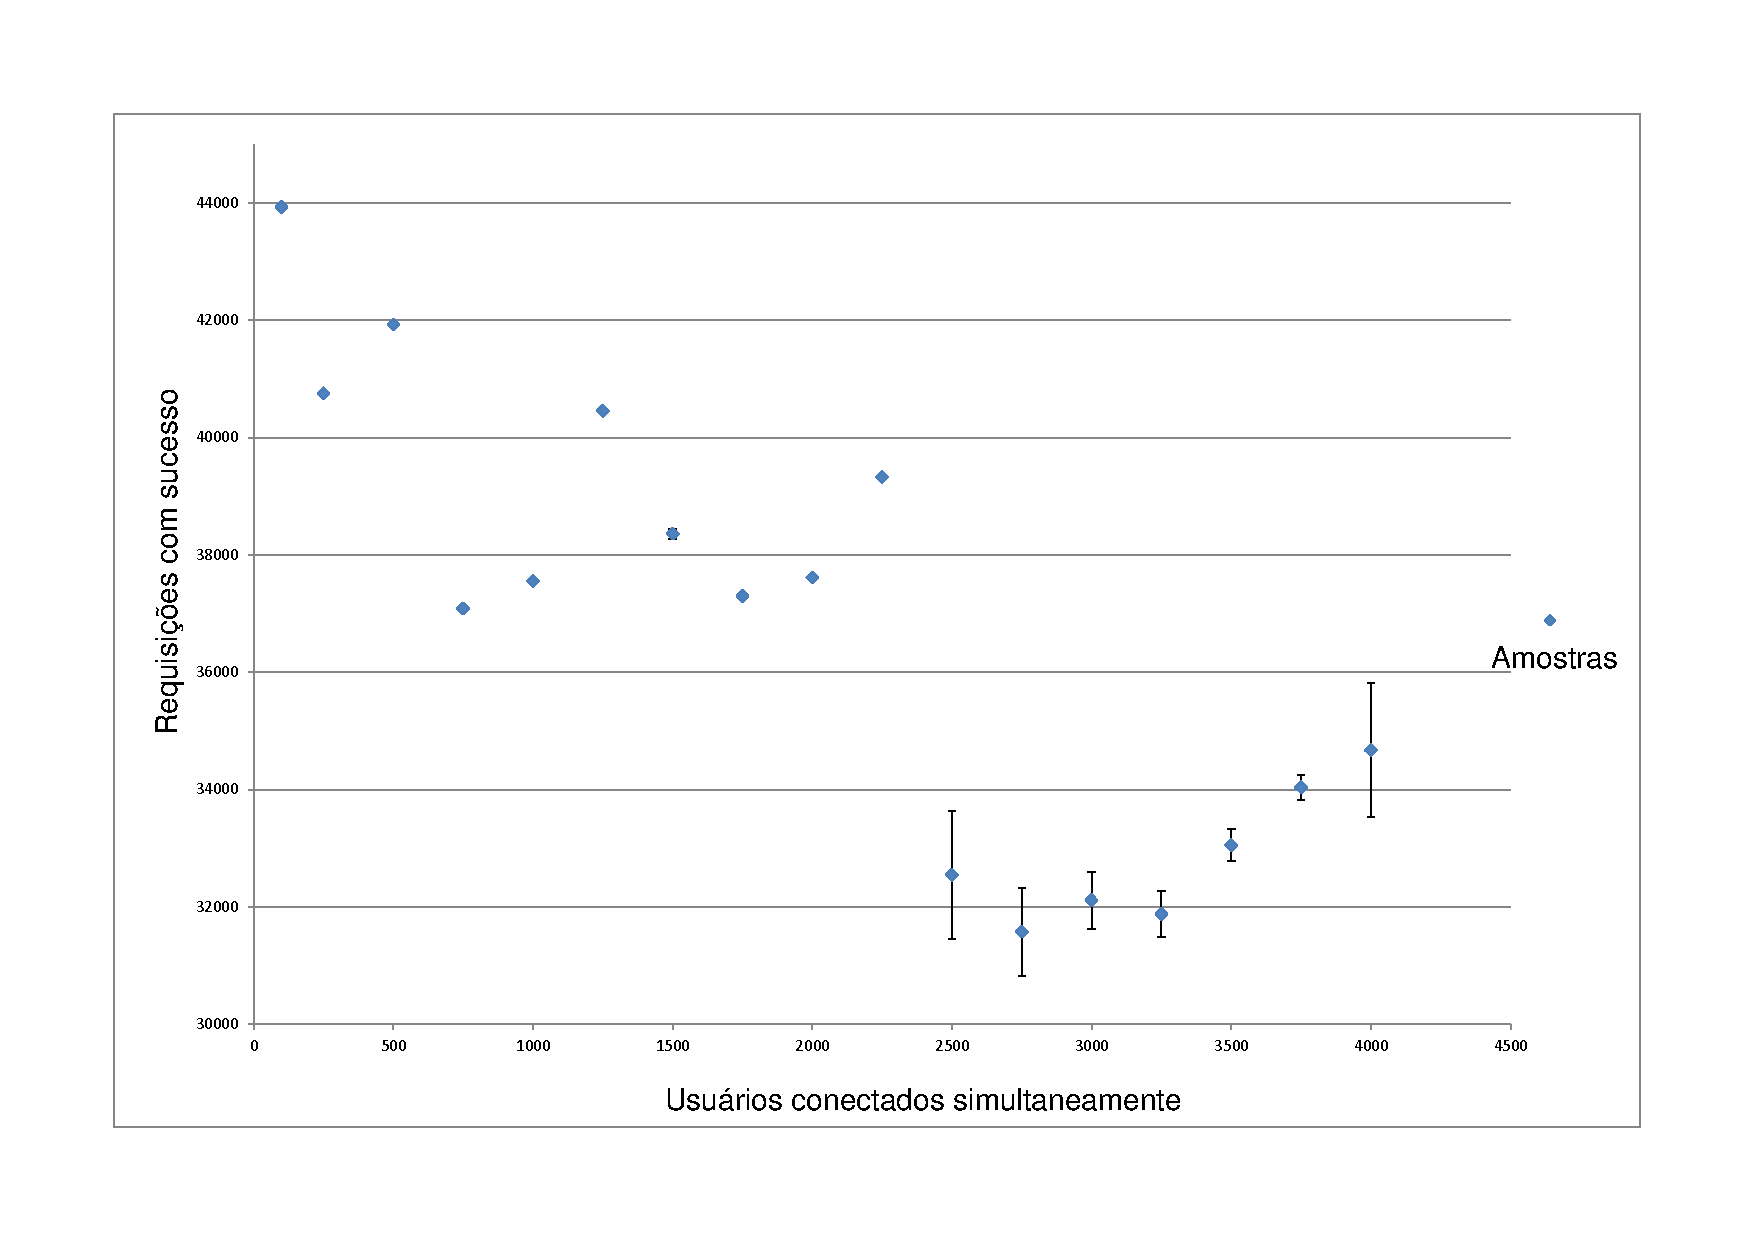
\includegraphics[scale=0.5]{imagens/dvp3.pdf}
    \caption{Média e desvio padrão do Cenário 3}
    \label{fig:dvp3}
    \end{figure}
    
        \begin{figure}[H]
    \centering
    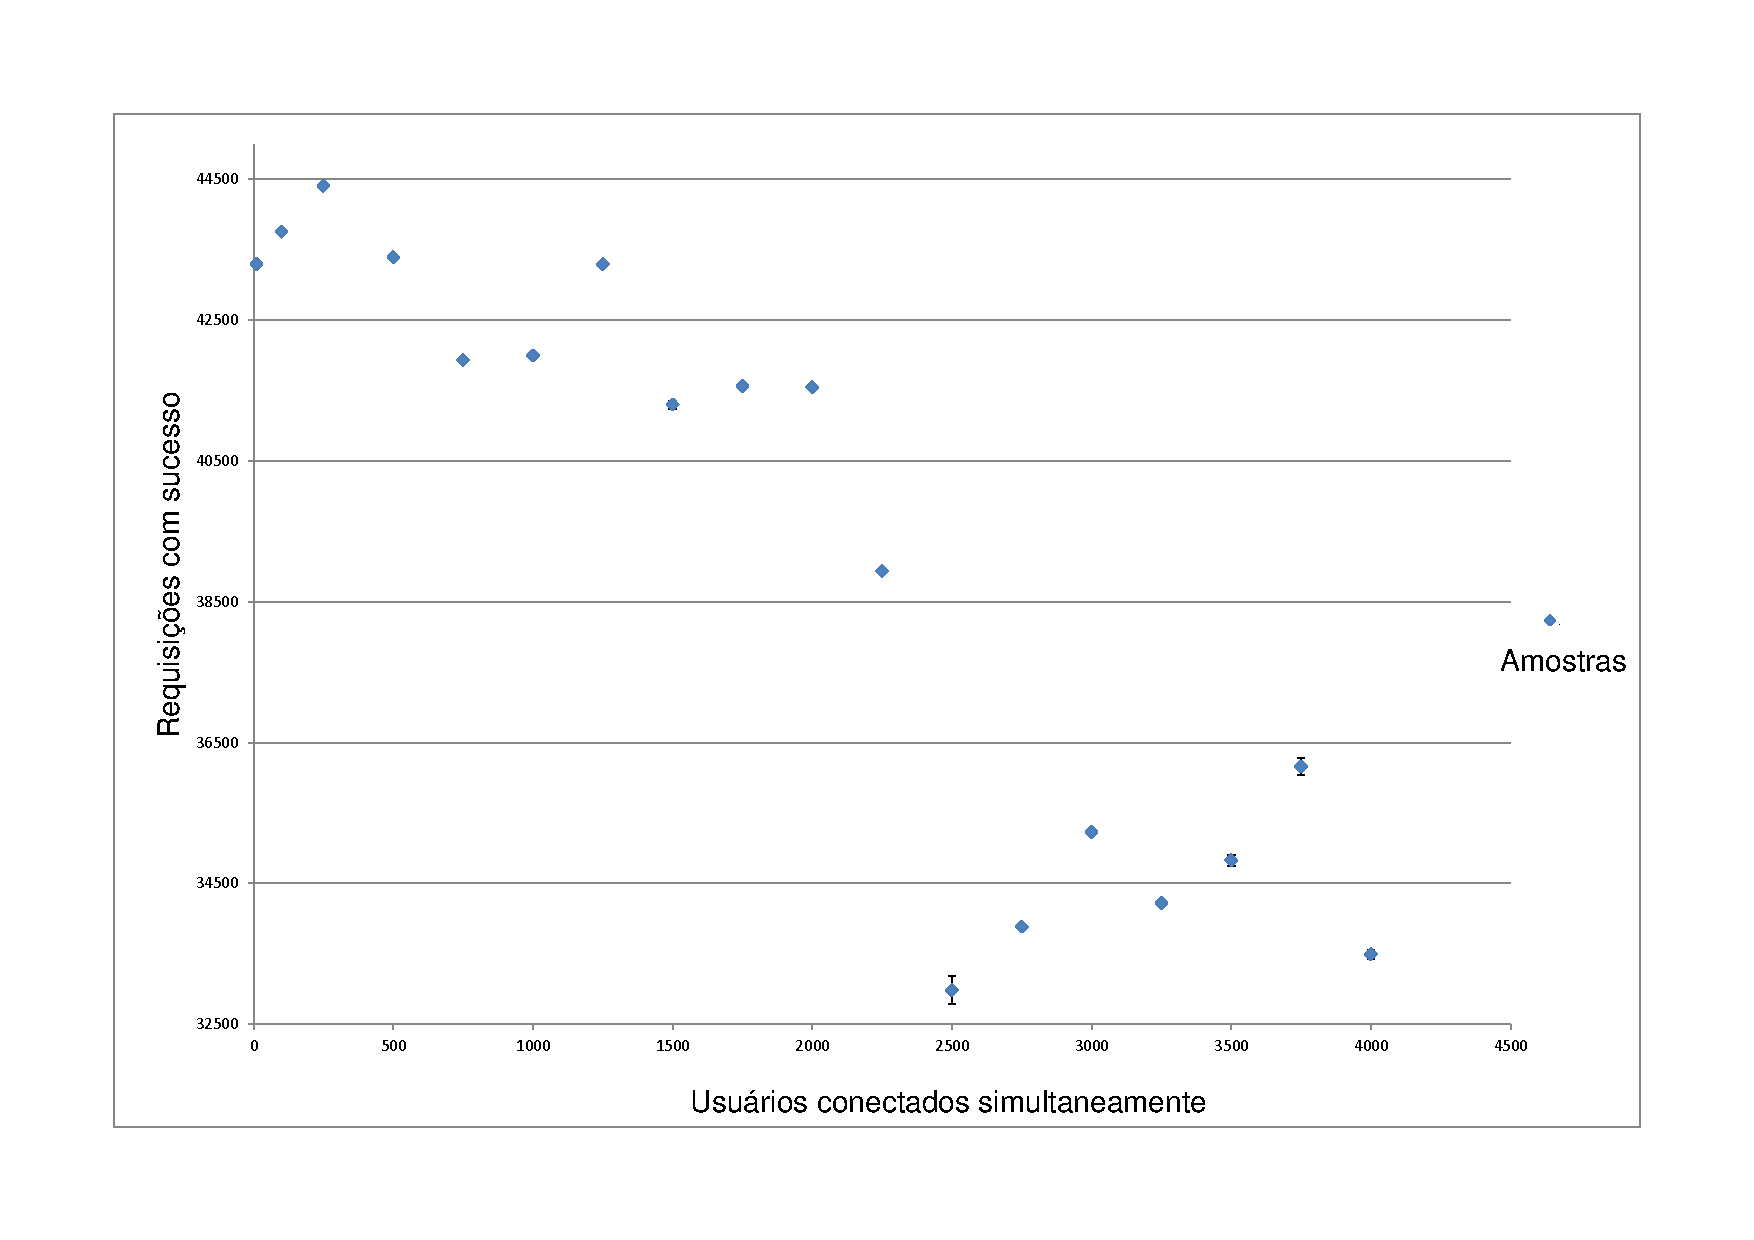
\includegraphics[scale=0.5]{imagens/dvp4.pdf}
    \caption{Média e desvio padrão do Cenário 4}
    \label{fig:dvp4}
    \end{figure}
    
        \begin{figure}[H]
    \centering
    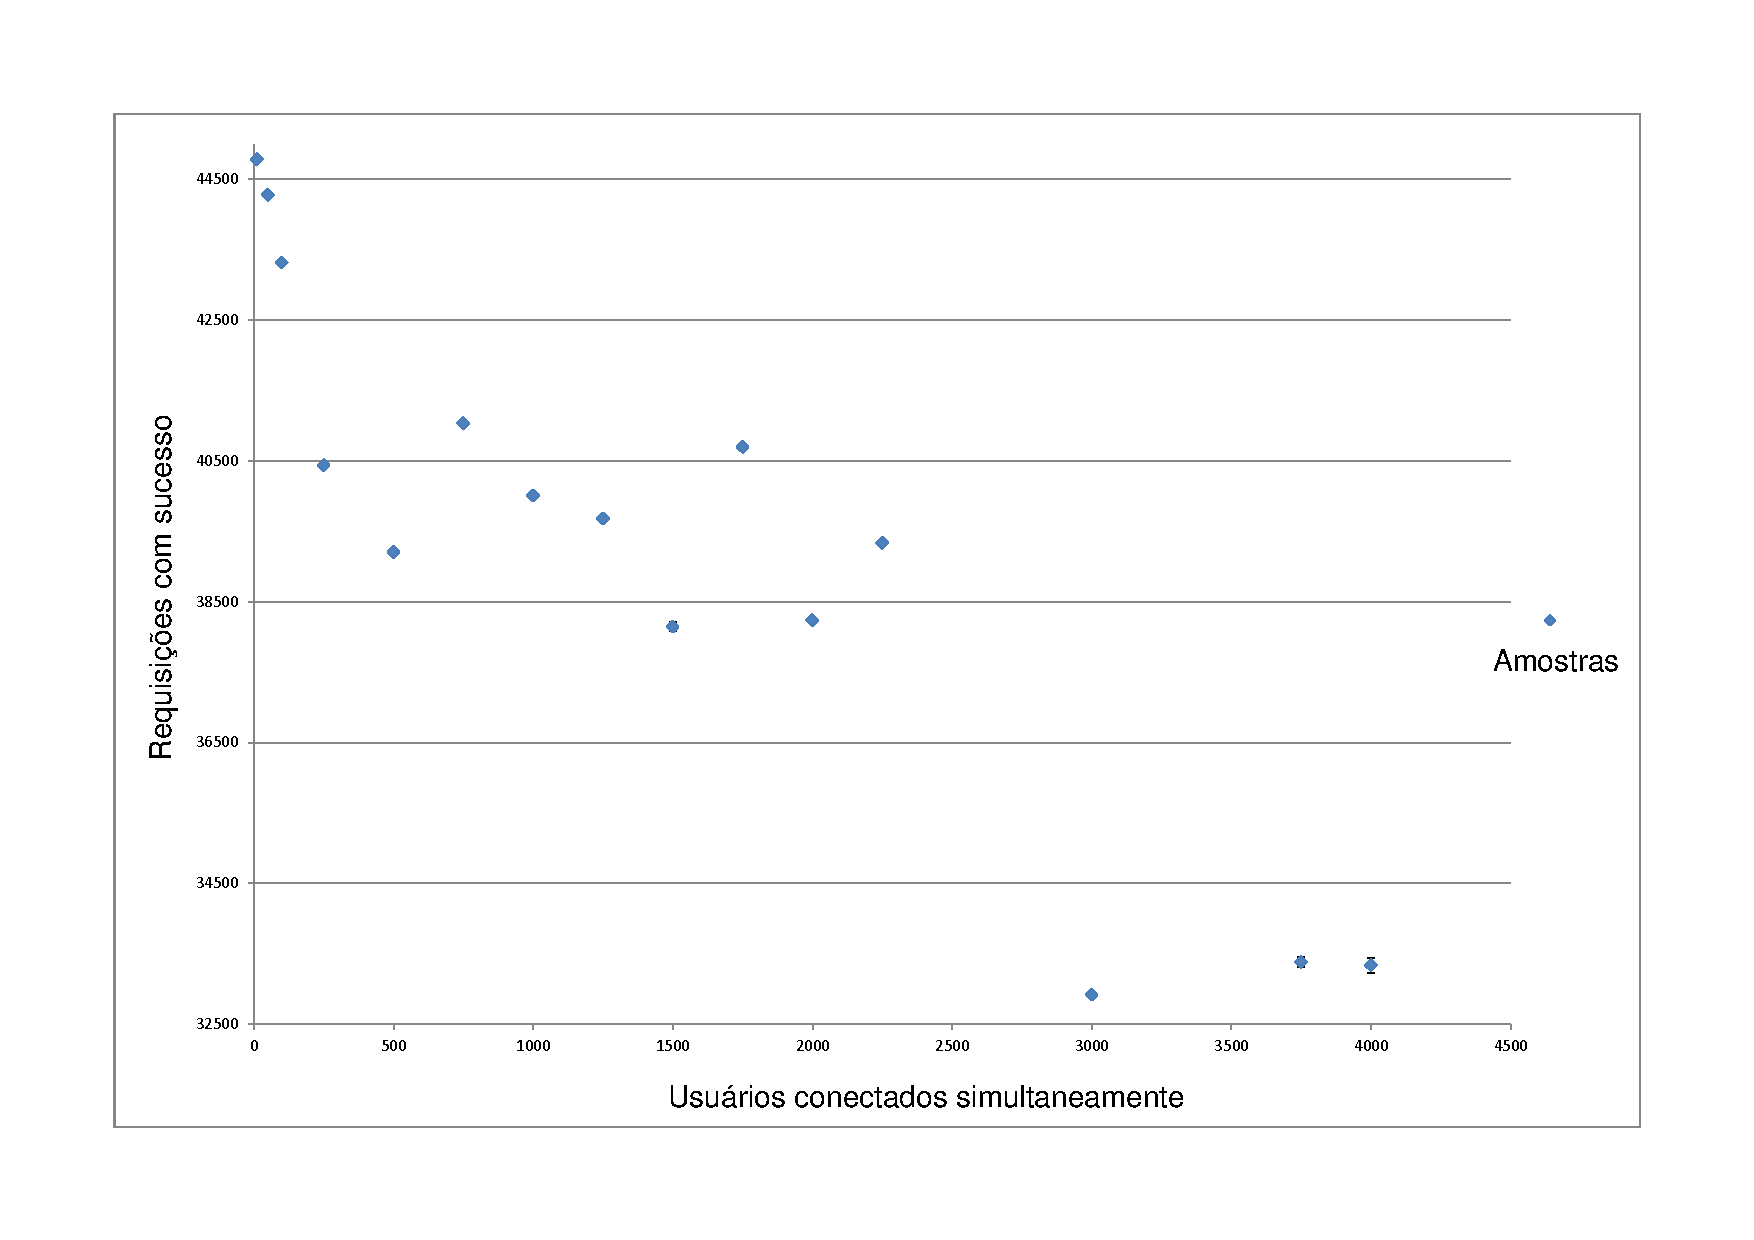
\includegraphics[scale=0.5]{imagens/dvp5.pdf}
    \caption{Média e desvio padrão do Cenário 5}
    \label{fig:dvp5}
    \end{figure}
    
    \begin{figure}[H]
    \centering
    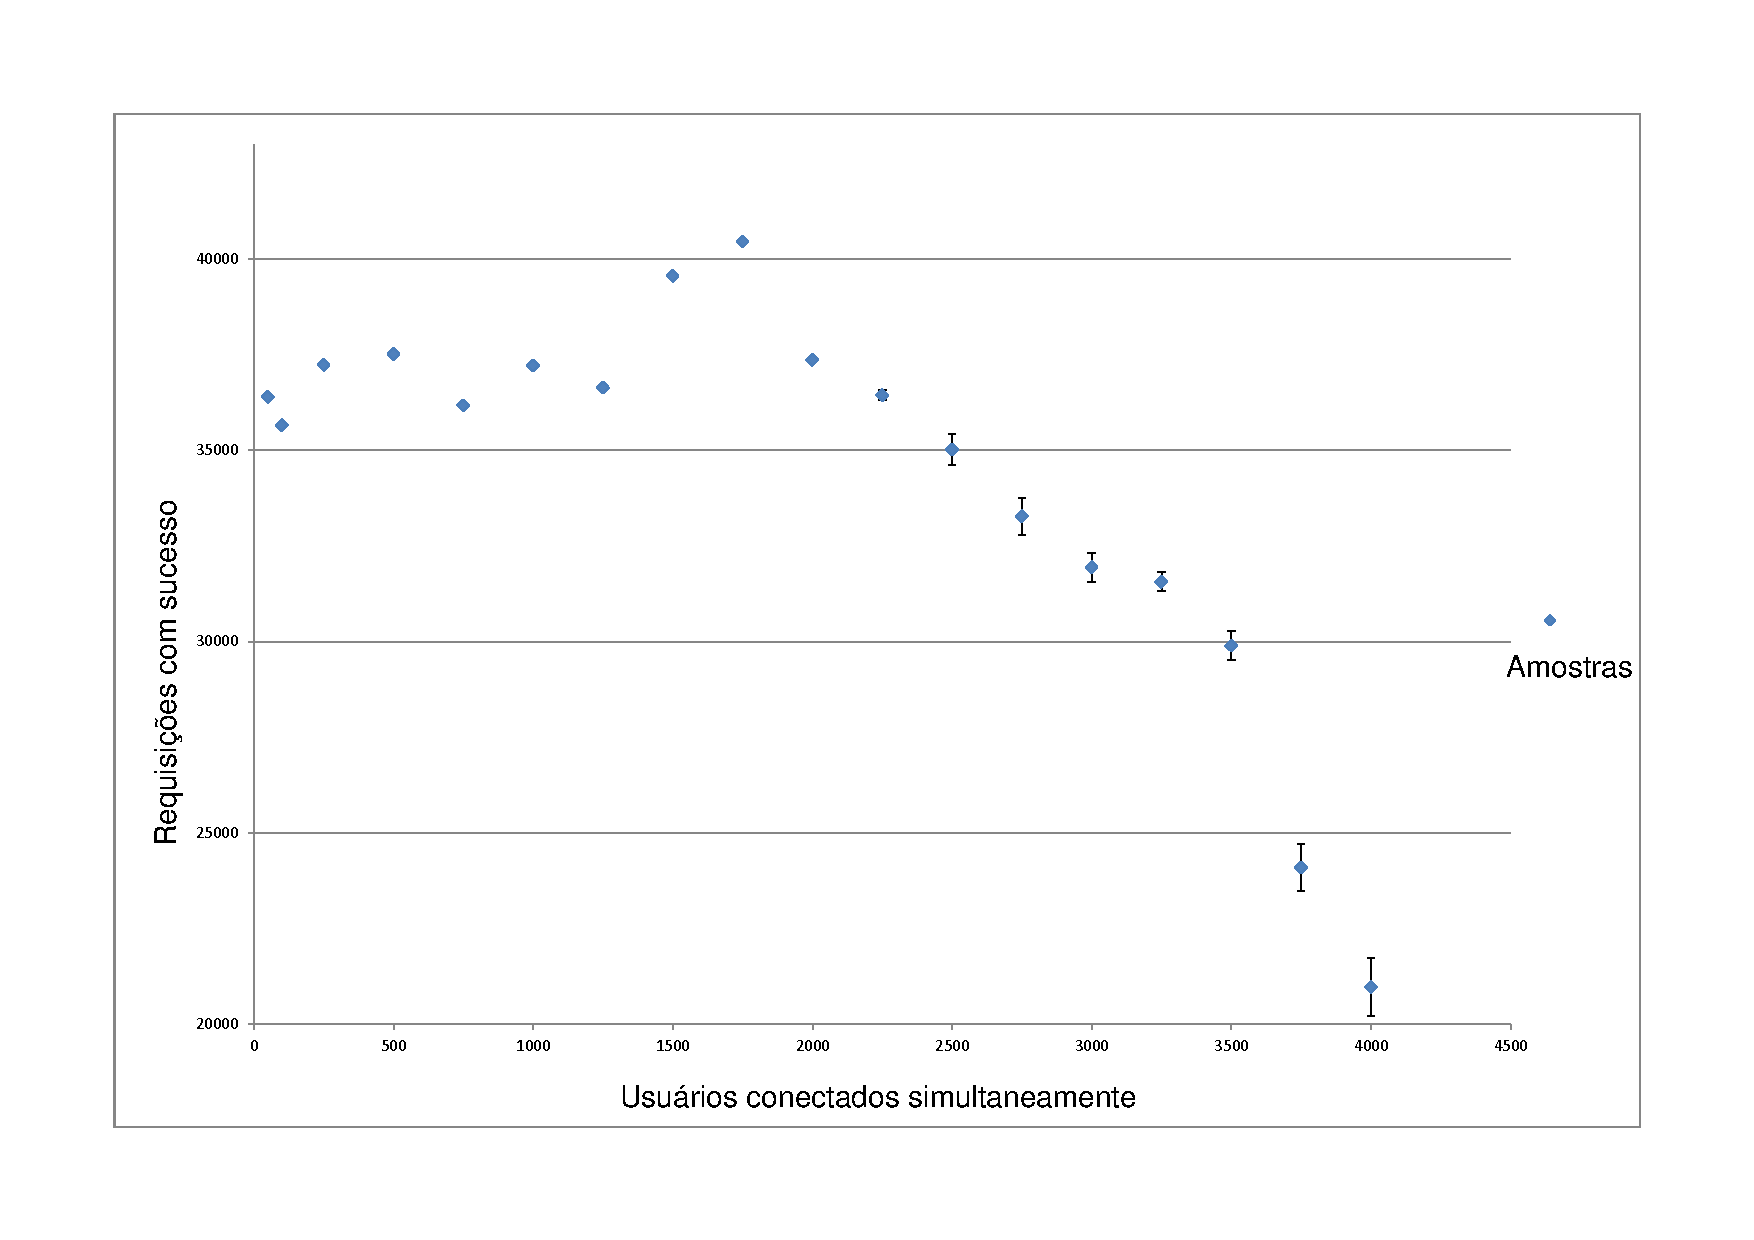
\includegraphics[scale=0.5]{imagens/dvp6.pdf}
    \caption{Média e desvio padrão do Cenário 6}
    \label{fig:dvp6}
    \end{figure}
    
Como a partir simulação com 2000 usuários praticamente todos os cenários aumentam o erro significativamente, considerou-se este o máximo que estes cenários suportam. Desta forma, plotou-se num gráfico a taxa de erro e a quantidade de requisições, onde observou-se que, nas simulações com até 2000 usuários, o erro é desconsiderável (< 0,1\%) em relação a quantidade de requisições atendidas com sucesso.

A Figura \ref{fig:max} ilustra esta simulação, cruzando total de requisições e porcentagem de erro em cada cenário, onde o erro sempre é menor que 0,1\%.    

    \begin{figure}[H]
    \centering
    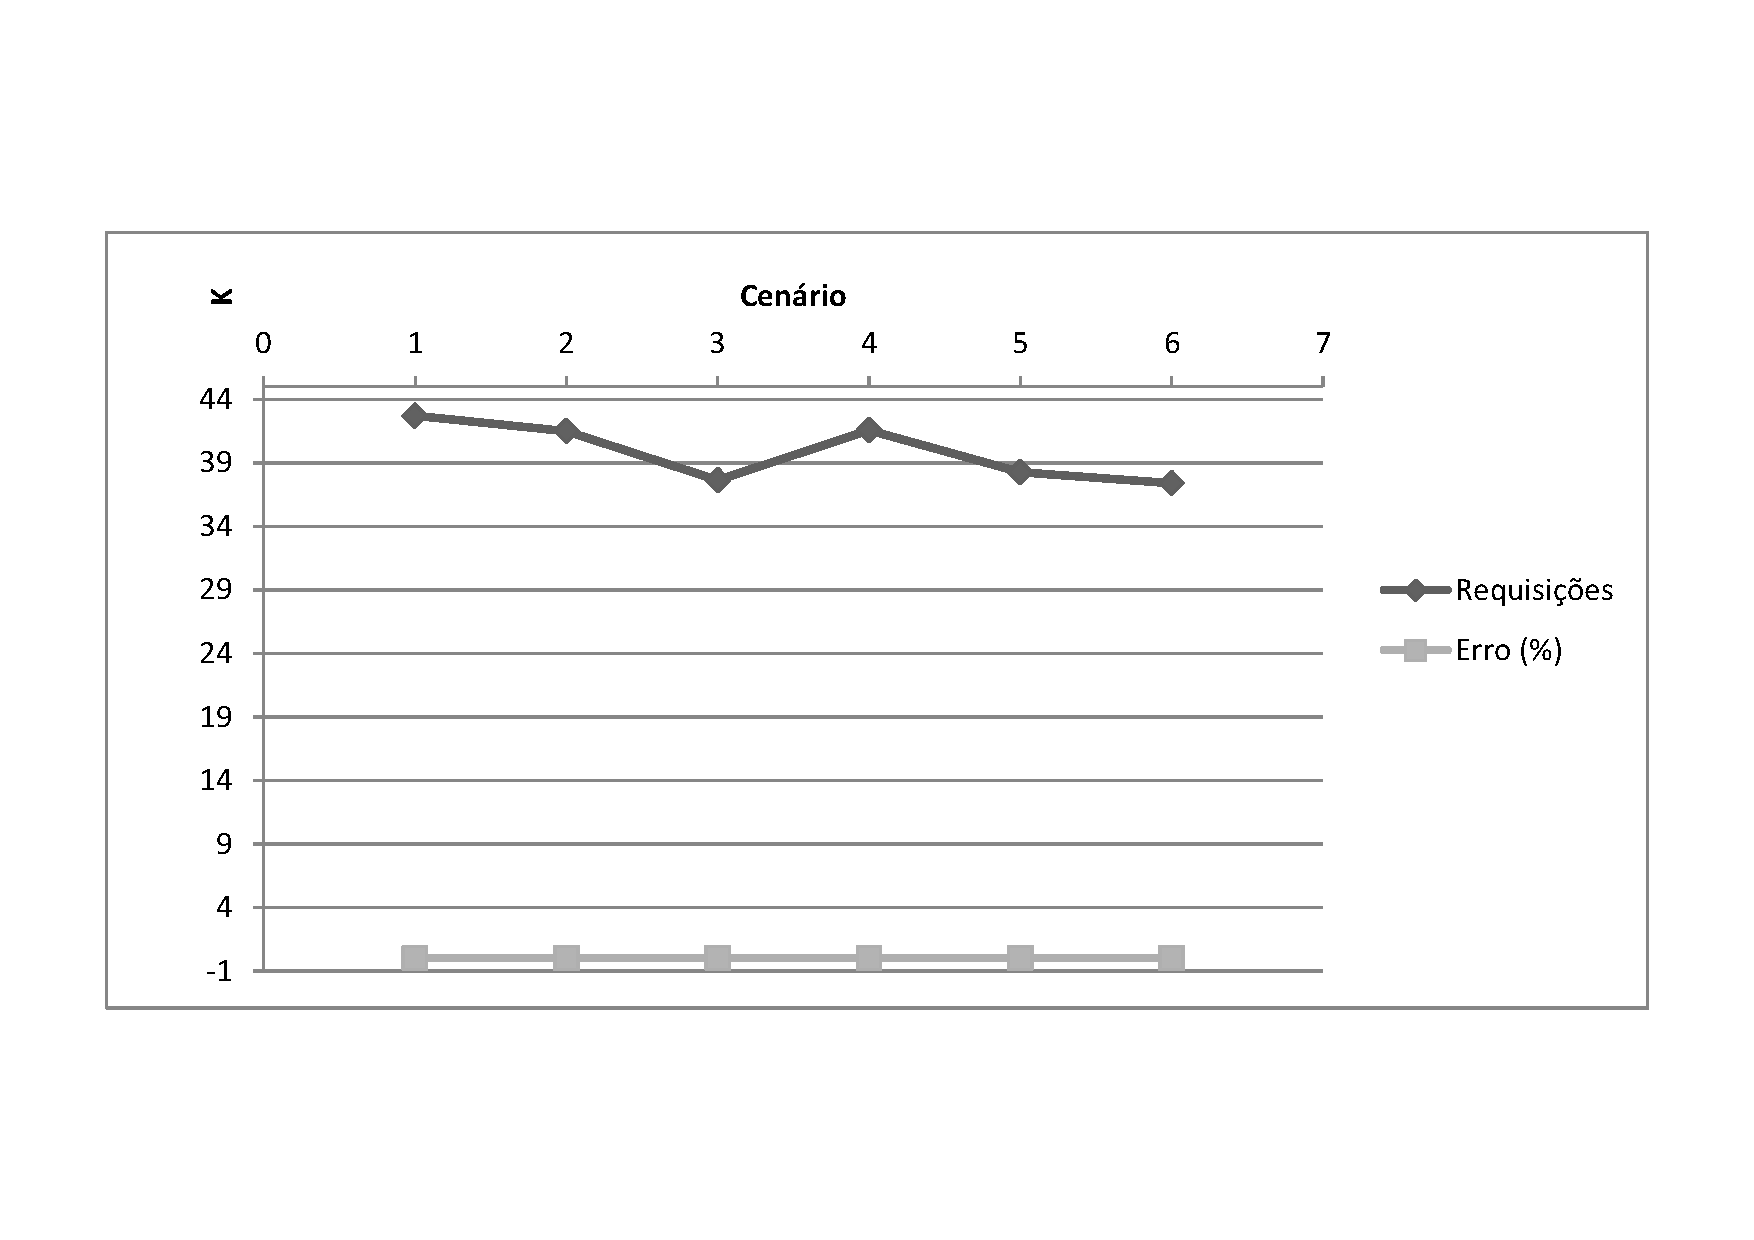
\includegraphics[scale=0.5]{imagens/reqXerro.pdf}
    \caption{Requisições e porcentagem de erro para 2000 usuários}
    \label{fig:max}
    \end{figure}

Por fim, foi estudado o impacto do uso de \textit{guests} na composição dos cenários, conforme Figura \ref{fig:lat}, que demonstrou que a latência das requisições nos cenários que não possuem \textit{guests} é menor. Porém, o uso de \textit{guests} na Computação em Nuvem traz diversos benefícios como abstração física de hardware, elasticidade, entre outros. A virtualização é o componente responsável pela característica dinâmica dos data centers. É através do uso das \textit{guests} que os ambientes virtuais de cada usuário podem ser ampliados ou reduzidos dinamicamente de maneira a atender aos recursos solicitados.  

    \begin{figure}[H]
    \centering
    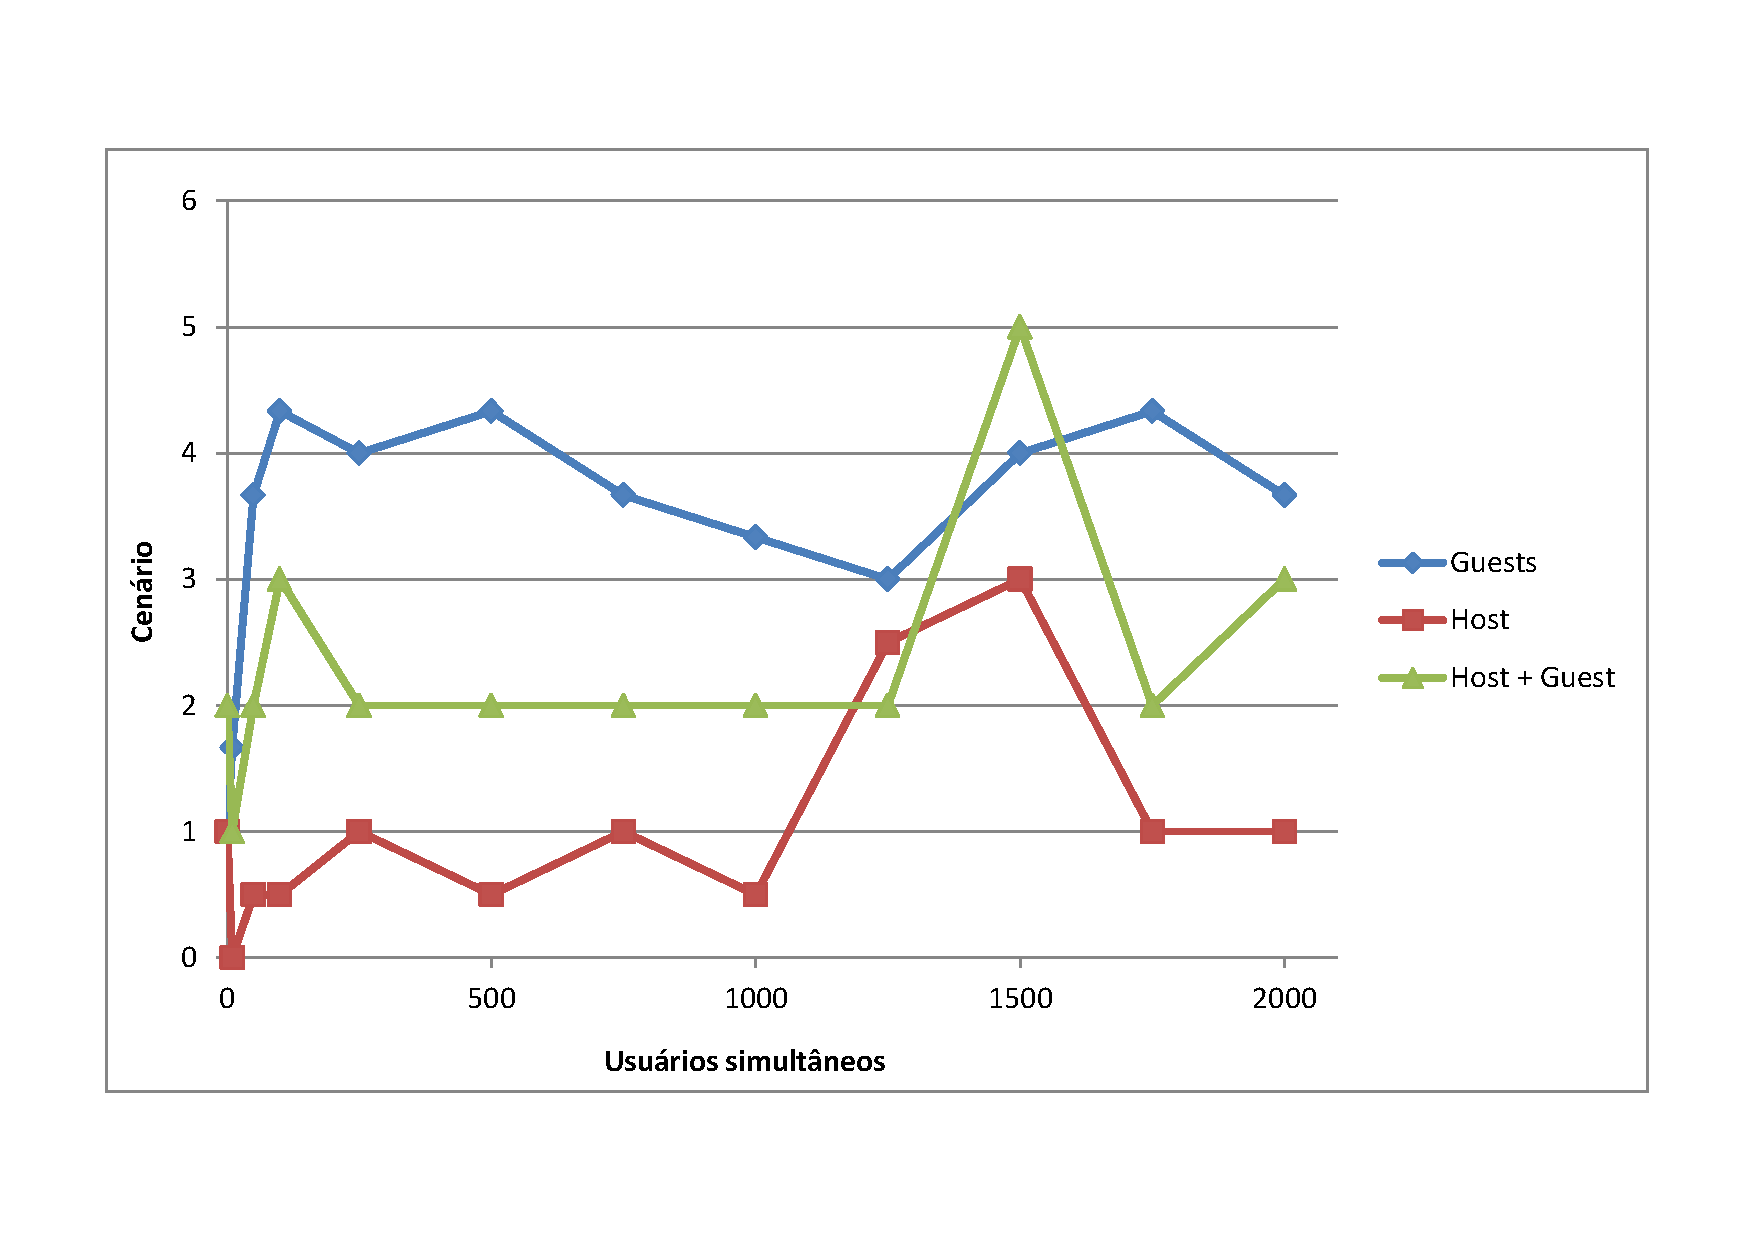
\includegraphics[scale=0.5]{imagens/latencia.pdf}
    \caption{Latência dos cenários de acordo com perfil de máquina utilizada}
    \label{fig:lat}
    \end{figure}

\section{Análise dos Resultados}
\label{sec:analResul}

Com o fim da realização das simulações e avaliação dos resultados, foi possível notar que a forma com que os cenários foram fisicamente implementados impactou na escalabilidade da base de dados. 

O Cassandra foi configurado na \textit{host} A e nesta mesma máquina foram instaladas 5 \textit{guests}. Destas, 4 eram dedicadas a base de dados e uma era responsável por executar e coletar os dados dos testes. Também havia uma \textit{host} B que fazia parte da base de dados, nos cenários em que mais de uma máquina física era necessária.

Sendo assim, sugere-se realizar em um futuro trabalho testes práticos com todas as ferramentas que o projeto Maritaca utiliza. Em especial, executar novos testes com o Cassandra, utilizando uma disposição diferente das máquinas onde a base de dados e a ferramenta responsável pelos testes estão instaladas.
